%!Mode:: "TeX:UTF-8"
\documentclass[a4paper,11pt,UTF8]{ctexart}

\usepackage{indentfirst} %缩进
\usepackage{xeCJK}    %使用系统字体
\usepackage{bm}       %粗体
\usepackage{fancyhdr} %自定义页眉页脚
\fancyhead[LE,RO]{~\thepage~} % 在偶数页的左侧,奇数页的右侧显示页码
\usepackage{amsmath, amsthm, amssymb, amsfonts} %数学公式
\usepackage[a4paper,left=3cm,right=3cm,top=3.5cm,bottom=3.5cm]{geometry}
\usepackage{booktabs} %插入表格
\usepackage[section]{placeins} %避免浮动
\usepackage{listings} %插入代码
\usepackage{ctex}     %中文宏包
\usepackage[svgnames, table]{xcolor} %彩色表格
\usepackage{algorithm}          %伪代码
\usepackage{algorithmicx}
\usepackage{algpseudocode}
\usepackage{algorithm,algpseudocode,float}
\usepackage{lipsum}
\usepackage{enumitem}           %调整列举环境
\usepackage{url}
\usepackage{fontspec,xunicode}
\usepackage{cite}
\defaultfontfeatures{Mapping=tex-text} %如果没有它,会有一些 tex 特殊字符无法正常使用,比如连字符。
\providecommand{\keywords}[1]{\textbf{\textit{Index terms---}} #1} %Keywords
%%%%%%%%%%%%%%%%%%%%%%%%%%%ABSTRACT%%%%%%%%%%%%%%%%%%%%%%%%%%%%%%%%%%%%%%%%%%
\newcommand{\enabstractname}{Abstract}
\newcommand{\cnabstractname}{摘 ~ 要}
\newenvironment{enabstract}{%
{\center \bfseries \enabstractname }
: %\!
}

\newenvironment{cnabstract}{%
{\center \bfseries \cnabstractname}
:%\!
}

\usepackage{graphicx}
\graphicspath{{imgs/}}

\usepackage{color}
\usepackage{transparent}
\usepackage{graphicx}
\usepackage{import}
% inkscape -D --export-type=pdf --export-latex process.svg


%%%%%%%%%%%%%%%%%%%%%%%%%%%%%%%%%%%%%%%%%%%%%%%%%%%%%%%%%%%%%%%%
% 缩进及行间距
%%%%%%%%%%%%%%%%%%%%%%%%%%%%%%%%%%%%%%%%%%%%%%%%%%%%%%%%%%%%%%%%
\setlength{\parindent}{22bp} %重新定义缩进长度
\linespread{1}

%%%%%%%%%%%%%%%%%%%%%%%%%%%%%%%%%%%%%%%%%%%%%%%%%%%%%%%%%%%%%%%%
% 图的标题行间距设置
%%%%%%%%%%%%%%%%%%%%%%%%%%%%%%%%%%%%%%%%%%%%%%%%%%%%%%%%%%%%%%%%
\newcommand{\bottomcaption}{%
\setlength{\abovecaptionskip}{6bp}%
\setlength{\belowcaptionskip}{6bp}%
\caption}


%%%%%%%%%%%%%%%%%%%%%%%%%%%%%%%%%%%%%%%%%%%%%%%%%%%%%%%%%%%%%%%%
% 字体定义
%%%%%%%%%%%%%%%%%%%%%%%%%%%%%%%%%%%%%%%%%%%%%%%%%%%%%%%%%%%%%%%%
\setmainfont{Times New Roman}  %默认英文字体.serif是有衬线字体sans serif无衬线字体
\setmonofont{Consolas}
\setCJKmainfont[ItalicFont={楷体}, BoldFont={黑体}]{宋体}%衬线字体 缺省中文字体为
\setCJKsansfont{宋体}
\punctstyle{hangmobanjiao}
%-----------------------xeCJK下设置中文字体------------------------------%
%\setCJKfamilyfont{song}{SimSun}                             %宋体 song
\let\SimSun\relax
\newCJKfontfamily\SimSun{SongTi}[AutoFakeBold]       %打开假粗体
\newcommand{\song}{\CJKfamily{song}}
\setCJKfamilyfont{fs}{FangSong}                      %仿宋  fs
\newcommand{\fs}{\CJKfamily{fs}} 
\let\kaishu\relax                                    %重定义楷体,打开假粗体
\newCJKfontfamily\kaishu{KaiTi}[AutoFakeBold] 
%\setCJKfamilyfont{ktgb}{KaiTi_GB2312}                      %楷体 GB2312
%\newcommand{\ktgb}{\CJKfamily{ktgb}}
\setCJKfamilyfont{yh}{Microsoft YaHei}                    %微软雅黑 yh
\newcommand{\yh}{\CJKfamily{yh}}
\setCJKfamilyfont{hei}{SimHei}                              %黑体  hei
\let\SimHei\relax
\newCJKfontfamily\SimHei{HeiTi}[AutoFakeBold]
\newcommand{\hei}{\CJKfamily{hei}}
\setCJKfamilyfont{hwxk}{STXingkai}                                %华文行楷  hwxk
\newcommand{\hwxk}{\CJKfamily{hwxk}}
%------------------------------设置字体大小------------------------%
\newcommand{\chuhao}{\fontsize{42bp}{63bp}\selectfont}     %初号, 1.5倍行距
\newcommand{\xiaochuhao}{\fontsize{36bp}{36bp}\selectfont} %小初号,单倍行距
\newcommand{\yihao}{\fontsize{26bp}{39bp}\selectfont}        % 一号, 1.5 倍行距
\newcommand{\erhao}{\fontsize{22bp}{33bp}\selectfont}        % 二号, 1.5倍行距
\newcommand{\xiaoerhao}{\fontsize{18bp}{18bp}\selectfont}       % 小二, 单倍行距
\newcommand{\sanhao}{\fontsize{16bp}{24bp}\selectfont}       % 三号, 1.5倍行距
\newcommand{\xiaosanhao}{\fontsize{15bp}{22bp}\selectfont}      % 小三, 1.5倍行距
\newcommand{\sihao}{\fontsize{14bp}{21bp}\selectfont}        % 四号, 1.5 倍行距
\newcommand{\banxiaosi}{\fontsize{13bp}{20bp}\selectfont}  % 半小四, 20pt行距
\newcommand{\xiaosihao}{\fontsize{12bp}{20bp}\selectfont}       % 小四, 20pt行距
\newcommand{\dawuhao}{\fontsize{11bp}{11bp}\selectfont}      % 大五号, 单倍行距
\newcommand{\wuhao}{\fontsize{10.5bp}{10.5bp}\selectfont}   % 五号, 单倍行距
\newcommand{\xiaowuhao}{\fontsize{9bp}{9bp}\selectfont}   %小五号,单倍行距
%------------------------------重定义normalize------------------------%
\renewcommand{\normalsize}{\fontsize{12bp}{20bp}\selectfont}


%%%%%%%%%%%%%%%%%%%%%%%%%%%%%%%%%%%%%%%%%%%%%%%%%%%%%%%%%%%%%%%%
% 图题字体大小相同
%%%%%%%%%%%%%%%%%%%%%%%%%%%%%%%%%%%%%%%%%%%%%%%%%%%%%%%%%%%%%%%%
\usepackage{caption}
\captionsetup{font={footnotesize}}   % footnotesize = 9bp
\captionsetup[lstlisting]{font={footnotesize}}

%%%%%%%%%%%%%%%%%%%%%%%%%%%%%%%%%%%%%%%%%%%%%%%%%%%%%%%%%%%%%%%%
% 重定义枚举编号为 1),2)...
%%%%%%%%%%%%%%%%%%%%%%%%%%%%%%%%%%%%%%%%%%%%%%%%%%%%%%%%%%%%%%%%
\renewcommand{\labelenumi}{\theenumi)}


%%%%%%%%%%%%%%%%%%%%%%%%%%%%%%%%%%%%%%%%%%%%%%%%%%%%%%%%%%%%%%%%
% 重定义section标题
%%%%%%%%%%%%%%%%%%%%%%%%%%%%%%%%%%%%%%%%%%%%%%%%%%%%%%%%%%%%%%%%
\CTEXsetup[format={\CJKfamily{zhhei}\zihao{4}},number={\chinese{section}},name={,、~},aftername={},indent={0bp},beforeskip={6bp},afterskip={6bp},format+={\flushleft}]{section}
% \CTEXsetup[format={\Large\bfseries\CJKfamily{zhkai}\zihao{5}},name={(,)},number={\chinese{subsection}},aftername={},indent={22bp},beforeskip={6bp},afterskip={6bp}]{subsection}
\CTEXsetup[number={\chinese{section}},name={附录, ~~ }]{appendix}



%%%%%%%%%%%%%%%%%%%%%%%%%%%%%%%%%%%%%%%%%%%%%%%%%%%%%%%%%%%%%%%%
% 标题名称中文化
%%%%%%%%%%%%%%%%%%%%%%%%%%%%%%%%%%%%%%%%%%%%%%%%%%%%%%%%%%%%%%%%
\renewcommand\figurename{\hei 图}
\renewcommand\tablename{\hei 表}
\renewcommand\lstlistingname{\hei 代码}
\renewcommand{\algorithmicrequire}{\textbf{输入:}}
\renewcommand{\algorithmicensure}{\textbf{输出:}}
\newtheorem{define}{定义}


%%%%%%%%%%%%%%%%%%%%%%%%%%%%%%%%%%%%%%%%%%%%%%%%%%%%%%%%%%%%%%%%
% 列表设置
%%%%%%%%%%%%%%%%%%%%%%%%%%%%%%%%%%%%%%%%%%%%%%%%%%%%%%%%%%%%%%%%
\setlist[enumerate,1]{itemindent=22bp,listparindent=\parindent,itemsep=0mm,partopsep=.7mm,parsep=0ex,labelsep=1.5mm,topsep=0.7mm}
\setlist[enumerate,2]{label=\alph*),leftmargin=1.5em}  %二级item设置
%\setitemize{itemindent=38bp,leftmargin=0bp,itemsep=-0.4ex,listparindent=26bp,partopsep=0bp,parsep=0.5ex,topsep=-0.25ex}
%\setdescription{itemindent=38bp,leftmargin=0bp,itemsep=-0.4ex,listparindent=26bp,partopsep=0bp,parsep=0.5ex,topsep=-0.25ex}

%%%%%%%%%%%%%%%%%%%%%%%%%%%%%%%%%%%%%%%%%%%%%%%%%%%%%%%%%%%%%%%%
% 代码设置
%%%%%%%%%%%%%%%%%%%%%%%%%%%%%%%%%%%%%%%%%%%%%%%%%%%%%%%%%%%%%%%%
\lstset{
 columns=fixed,
 numbers=left,                                        % 在左侧显示行号
 numberstyle=\tiny\color{gray},                       % 设定行号格式
 frame=single,                                        % 单线背景边框
 breaklines=true,                                     % 设定LaTeX对过长的代码行进行自动换行
 keywordstyle=\color[RGB]{40,40,255},                 % 设定关键字颜色
 numberstyle=\footnotesize\color{darkgray},
 commentstyle=\it\color[RGB]{0,96,96},                % 设置代码注释的格式
 stringstyle=\rmfamily\slshape\color[RGB]{128,0,0},   % 设置字符串格式
 showstringspaces=false,                              % 不显示字符串中的空格
 language=java,                                        % 设置语言
 basicstyle=\linespread{1.0}\xiaowuhao\ttfamily,                      % 字体字号
 %lineskip=10bp,
 %baselinestretch=1,
}

%%%%%%%%%%%%%%%%%%%%%%%%%%%%%%%%%%%%%%%%%%%%%%%%%%%%%%%%%%%%%%%%
% 伪代码分页
%%%%%%%%%%%%%%%%%%%%%%%%%%%%%%%%%%%%%%%%%%%%%%%%%%%%%%%%%%%%%%%%
\makeatletter
\renewcommand{\ALG@name}{算法}
\newenvironment{breakablealgorithm}
  {% \begin{breakablealgorithm}
   \begin{center}
     \refstepcounter{algorithm}% New algorithm
     \hrule height.8bp depth0bp \kern2bp% \@fs@pre for \@fs@ruled
     \renewcommand{\caption}[2][\relax]{% Make a new \caption
       {\raggedright\textbf{\ALG@name~\thealgorithm} ##2\par}%
       \ifx\relax##1\relax % #1 is \relax
         \addcontentsline{loa}{algorithm}{\protect\numberline{\thealgorithm}##2}%
       \else % #1 is not \relax
         \addcontentsline{loa}{algorithm}{\protect\numberline{\thealgorithm}##1}%
       \fi
       \kern2bp\hrule\kern2bp
     }
  }{% \end{breakablealgorithm}
     \kern2bp\hrule\relax% \@fs@post for \@fs@ruled
   \end{center}
  }
\makeatother


\begin{document}
\xiaosihao\song

\begin{titlepage}
  \vspace{4cm}
  % \center\includegraphics[width=\textwidth]{logo}
  \center{\xiaochuhao{设计报告}}

  \vspace{6cm}

  \center{\sanhao{Author: innns}}


\end{titlepage}
\clearpage


\begin{center}
  \begin{large}
    \yihao{\hei{智能物流搬运机器人视觉及通信系统设计}}
  \end{large}
\end{center}
\begin{center}
  $\divideontimes$ innns
\end{center}

\begin{cnabstract}
  智能物流搬运机器人适用于各种仓库、车间中物料的搬运,能够大大减少仓库、车间中对人力的需求。由于成本低、生产周期短,因此能够大规模的批量生产,也能普遍应用。
  作者随队参加的第七届全国大学生工程训练综合能力竞赛-智能+赛道赛事中,我们队伍设计了一个智能物流搬运机器人,模拟工厂制造过程,实现了机器人利用陀螺仪、编码器、以及巡线模块自主定位导航;读取二维码或利用WiFi通信获取搬运任务;以及利用视觉识别自动地高精度地搬运、存放物料等功能。
  {\center \bfseries 关键字:搬运机器人、计算机视觉}
\end{cnabstract}

\newpage
\tableofcontents
\newpage
%\clearpage

\section{绪论}
随着电子信息技术的高速发展,机器人在越来越多的领域协助人们更好的工作。其中物流机器人在如今的仓库管理中的作用愈发凸显。物流机器人涉及的核心技术包括导航及定位技术、运动控制技术、计算机视觉技术等。
\subsection{智能机器人设计需求}
\subsubsection{功能要求}
我们自主设计并制作一台按照给定任务完成物料搬运的智能机器人(简称:机器人)具有定位、移动、避障、读取条形码及二维码、Wi-Fi网络通信、物料位置和颜色识别、物料抓取与载运、上坡和下坡、路径规划等功能;竞赛过程机器人可以自主运行,或采用无线人机交互手段操作,但必须首选自主运行方式,只有在自主运行方式出现故障时才可申请使用无线遥控运行方式。该机器人能够通过扫描二维码或 Wi-Fi网络通信等方式领取搬运任务,在指定的工业场景内行走与避障,并按任务要求将物料搬运至指定地点并精准摆放(色环或条形码)。
\subsubsection{电控及驱动要求}
机器人所用传感器和电机的种类及数量不限,在机器人的醒目位置安装有任务码显示装置,显示装置必须放置在机器人上部醒目位置,且不被任何物体遮挡,必须是亮光显示,字体高度不小于8mm,该装置能够持续显示所有任务信息直至比赛结束,否则成绩无效。机器人各机构只能使用电驱动,采用电池(蓄电池除外)供电,供电电压限制在12V以下,随车装载,比赛过程中不能更换。
\subsubsection{机械结构要求}
自主设计并制造机器人的机械部分,除标准件外,非标零件应自主设计和制作,不允许使用购买的成品套件拼装而成。机器人的行走方式、机械手臂的结构形式均不限制,机器人腕部与手爪的连接结构自行确定。
\subsubsection{外形尺寸及载重要求}
机器人(含机械手臂)外形尺寸满足铅垂方向投影在边长为 300mm 的正方形内,高度不超过 400mm 方可参加比赛。允许机器人结构设计为可折叠形式,但出发之后才可自行展开。在初赛时机器人没有载重要求,而在决赛时机器人的总重量不能小于规定重量,用于对集成在决赛场地中的桥梁进行测试。载重物块形状自定,运行时物块不能掉落。
\subsection{运行环境}
\subsubsection{机器人运行场地}
近水平铺设的赛场尺寸为 $4800\times2400~mm$长方形平面区域(如图 \ref{fig_Field}),
\begin{figure}[htbp]
  \centering
  \includegraphics[width=12cm]{场地.jpg}
  \caption{场地示意图} \label{fig_Field}
\end{figure}
赛场周围设有一定高度的挡板,仅作为场地边界(颜色和高度不做任何要求),不宜作为寻边等其它任何用途。赛道地面为亚光白色或浅黄色等浅色底色,地面图案由线宽为 $20~mm$、线中心距为 $300~mm$ 的黑色方格组成。在比赛场地内,设置出发区、返回区、原料区、粗加工区、半成品区、精加工区、库存区。

其中机器人初赛主要经过原料区、粗加工区和半成品区完成粗加工物料的搬运过程;机器人决赛主要经过半成品区、精加工区和库存区完成精加工物料的搬运过程。出发区和返回区的尺寸均为$300\times300~mm$,颜色分别为蓝色和褐色;原料区和库存区的尺寸(长$\times$宽$\times$高)为 $580\times145\times(80-100)~mm$白色亚光的双层货架(原料区的高度为$100~mm$,物料采用颜色识别,库存区的货架高度在$80-100~mm$范围 ,采用条形码识别物料放置的位置)(如图 \ref{fig_Material_F}所示)
\begin{figure}[ht]
  \centering
  \includegraphics[width=12cm]{原料区.jpg}
  \caption{原料区示意图} \label{fig_Material_F}
\end{figure}
粗加工区和精加工区的尺寸(长$\times$宽)为 $580\times150~mm$;半成品区的尺寸(长$\times$宽$\times$高)为 $580\times150\times45$ 及 $580\times148\times0~mm$的台阶区域(如图 \ref{fig_Half} 所示)
\begin{figure}[htbp]
  \centering
  \includegraphics[width=12cm]{半成品区.jpg}
  \caption{半成品区示意图} \label{fig_Half}
\end{figure}
粗加工区、半成品区、精加工区顶面上均有用于测量物料摆放位置准确程度的色环,色环如图\ref{fig_Target} \ref{fig_Target_} 所示,其中$\phi$ 为物料最大直径(单位:$mm$),$\phi 1 — \phi 5$ 为色环 $1-5$ 环的外径,色环线宽为 $1.5~mm$。除标注尺寸外,其余色环的直径差为 $10~mm$。库存区顶面有外径为$\phi$(物料直径)$+15~mm$ 的圆形区域,用于确定物料是否摆放到位。

\begin{figure}[htbp]
  \begin{center}
    \begin{minipage}[t]{0.45\linewidth}
      \centering
      \includegraphics[height=6cm]{色环.jpg}
      \caption{色环尺寸图}\label{fig_Target}
    \end{minipage}%
    \begin{minipage}[t]{0.45\linewidth}
      \centering
      \includegraphics[height=6cm]{色环_.jpg}
      \caption{色环示意图}\label{fig_Target_}
    \end{minipage}
  \end{center}
\end{figure}


\subsubsection{物料}
机器人初赛时待搬运的物料形状包络在直径为 $50~mm$、高度为 $70~mm$、重约为$50~g$ 的圆柱体中(如图 \ref{fig_Material} 所示),夹持部分的形状为球体,物料的材料为 3D 打印ABS,三种颜色为:红(ABS/Red(C-21-03))、绿(ABS/Green(C-21-06))、蓝(ABS/Blue(C-21-04))。三种不同颜色的物料(每种颜色两个)随机放置在原料区的物料架上(上层及下层红、绿、蓝物料各一个),物料间距为 $150~mm$(如图 \ref{fig_Material_F} 所示)
\begin{figure}[htbp]
  \centering
  \includegraphics[width=6.5cm]{物料.jpg}
  \caption{原料示意图} \label{fig_Material}
\end{figure}

\newpage

\subsubsection{总体设计}
总体设计如图\ref{fig_car_sw},上层使用二维平台,实现垂直、水平移动;通过DJI 3508电机实现上层结构旋转;通过DJI 2006电机实现手抓升降;通过舵机实现手抓开闭;其中机器人拥有OV2710,OV5647两个相机分别对准前方和地面。
\begin{figure}[htbp]
  \centering
  \includegraphics[height=6.5cm]{car_sw.jpg}
  \includegraphics[height=6.5cm]{car_cam.jpg}
  \caption{总体设计图} \label{fig_car_sw}
\end{figure}



\section{设计方案论证}
\subsection{视觉系统}
目前主流的较低成本(1000元以下)的嵌入式视觉解决方案主要有OpenMV、FPGA、树莓派、Nvidia Jetson Nano等。其中:
\begin{itemize}
  \item OpenMV,简单来说,它是一个可编程的摄像头,摄像头本身内置了一些图像处理算法,很容易使用\cite{OpenMV},价格也较低(400-700元)。
  \item FPGA相比CPU处理图像而言具有并发处理的优势,但是实现较为困难,扩展性差。
  \item 树莓派(图\ref{fig_Pi})是一款基于ARM的微型电脑主板,以SD/MicroSD卡为内存硬盘。树莓派4B拥有内置无线网卡、40-pin GPIO、2个USB3.0及2个USB2.0、具备HDMI输出功能,可扩展性强,性能较好。价格较低(当时2GB版本300元,2022年1月国内竟然卖到了600元以上...)
  \item Nvidia Jetson Nano Developer Kit(图\ref{fig_Nano}是英伟达对标树莓派出品的一款基于ARM的边缘计算设备。性能高于树莓派,可扩展性也稍微强于树莓派(拥有4个USB3.0,且兼容树莓派40-pin GPIO,可安装m.2接口外置天线的无线网卡)。但是由于各种原因,官网2GB版本69美元、4GB版本99美元的价格到了国内(2022年1月)变成了850元和1300元左右。
\end{itemize}

\begin{figure}[htbp]
  \begin{center}
    \begin{minipage}[t]{0.45\linewidth}
      \centering
      \includegraphics[width=6cm]{Pi.jpg}
      \caption{树莓派} \label{fig_Pi}
    \end{minipage}%
    \begin{minipage}[t]{0.45\linewidth}
      \centering
      \includegraphics[width=6cm]{nano.jpg}
      \caption{Jetson Nano} \label{fig_Nano}
    \end{minipage}
  \end{center}
\end{figure}

\subsection{WiFi通信}
WiFi通信可以选择的方案并不多,除了内置WiFi的树莓派或者可装WiFi模块的Jetson Nano,还可以选择WiFi串口模块或带有WiFi功能的单片机如ESP系列实现UDP和服务器通信。

\subsection{选型}
综合以上考虑我们选择了基于树莓派的方案(图\ref{fig_Pi})。采用了一款体积较大,传感器为OV2710,1/2.7英寸CMOS的USB工业相机用于识别物料的颜色(图\ref{fig_Cam_C});一款体积较小,传感器为OV5647,1/4英寸CMOS的USB相机用于识别并定位靶子(图\ref{fig_Cam_T})。


\begin{figure}[htbp]
  \begin{center}
    \begin{minipage}[t]{0.45\linewidth}
      \centering
      \includegraphics[width=6cm]{颜色摄像头.jpg}
      \caption{颜色摄像头}\label{fig_Cam_C}
    \end{minipage}%
    \begin{minipage}[t]{0.45\linewidth}
      \centering
      \includegraphics[width=6cm]{靶子摄像头.jpg}
      \caption{靶子摄像头}\label{fig_Cam_T}
    \end{minipage}
  \end{center}
\end{figure}

\section{系统设计方案}
\subsection{系统硬件环境}
\begin{itemize}
  \item Raspberry Pi 4B 2GB (图\ref{fig_Pi})
  \item OV2710 USB camera(图\ref{fig_Cam_C})
  \item OV5647 USB camera(图\ref{fig_Cam_T})
\end{itemize}
\subsection{系统软件环境}
\begin{itemize}
  \item 2021-05-27-raspios-buster-arm64
  \item OpenCV 4.5.2 + contrib
  \item C++
  \item CMake
\end{itemize}

\newpage

\subsubsection{相机端口绑定}
由于重启之后相机端口号可能会改变,故使用v4l/by-id的软链接绑定相机端口号。
\begin{lstlisting}[caption={相机端口绑定},captionpos=b]
# e.g.
# ll /dev/v4l/by-id 再用软链接绑定
ll /dev/v4l/by-id 
# $ tree /dev/v4l
# /dev/v4l
# ├── by-id
# │   └── usb-OmniVision._USB_Camera-B4.04.27.1-video-index0 -> ../../video0
# └── by-path
#     └── pci-0000:00:14.0-usb-0:2:1.0-video-index0 -> ../../video0
sudo ln -s /dev/v4l/by-id/usb-337b_HBVCAM_5M-AF-video-index0 /dev/camera1
\end{lstlisting}

\subsection{开发环境}
作者使用了Windows 10 + VS Code 通过SSH连接树莓派开发,插件如下:
\begin{itemize}
  \item ms-vscode.cpptools-extension-pack
  \item coenraads.bracket-pair-colorizer
  \item obkoro1.korofileheader
  \item christian-kohler.path-intellisense
  \item ms-python.python
  \item gruntfuggly.todo-tree
  \item visualstudioexptteam.vscodeintellicode
  \item donjayamanne.githistory
  \item eamodio.gitlens
  \item github.vscode-pull-request-github
\end{itemize}
并且也使用了WSL在Ubuntu amd64环境下验证代码。

\newpage

\subsection{系统总体流程}
主程序会单独开一个监听线程实时监听32串口,当32发送命令时,若判断命令格式正确则会执行相应命令的功能。图\ref{fig_Process}即为系统流程图。因为扫颜色使用OV2710,扫靶子使用OV5647,为减小性能损失一次只打开一个相机,故需要切换相机功能。其中串口代码使用了Ge Zhenpeng学长的rmoss\_core,Github @gezp,Apache2.0协议\cite{UART};WiFi通信部分使用了 Github @eminfedar的async-sockets-cpp,MIT协议\cite{Socket},在此致谢。
\begin{figure}[htbp]
  \centering
  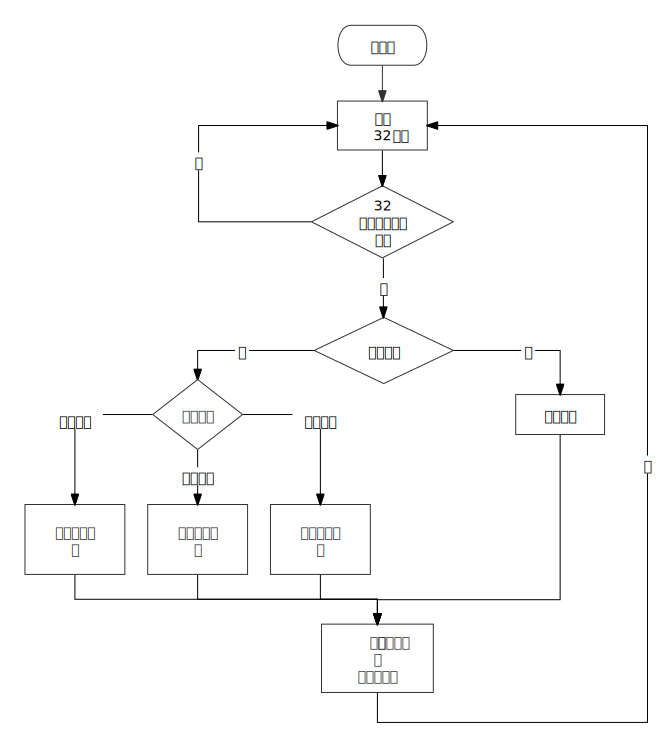
\includegraphics{process.pdf}
  \caption{系统流程图}\label{fig_Process}
\end{figure}

\subsection{通信系统}
\subsubsection{串口通信}
\paragraph{数据帧封装}
采用16字节数据帧,采用小端模式,封装如下:
\begin{table}[!ht]
  \begin{tabular}{|l|l|l|l|l|}
  \hline
      帧头*1 & 命令位*1 & 数据位*12 & 校验位*1 & 帧尾*1 \\ \hline
      [0] 0xAA & [1] CMD & [2-13] DATA & [14] 0xF0 & [15] 0xBB \\ \hline
  \end{tabular}
\end{table}

\paragraph{协议定义}
具体定义如下:
\begin{lstlisting}[caption={相机端口绑定},captionpos=b]
typedef enum : unsigned char
{
    // >>>>>> 发送用
    CMD_CURRENT_COLOR = 0x01, // 当前检测到的颜色 条形码读取的颜色
    CMD_TARGET_POS = 0x02,    // 当前检测到的靶心
    CMD_QR_MISSION = 0x03,    // 二维码读取的任务
    CMD_ALL_COLOR = 0x04,     // 所有颜色读取
    CMD_ACK = 0x05,           // 确认 切换相机 切换靶心等
    CMD_STORE_POS = 0x06,     // 库存区域位置

    // >>>>>> 接收用
    CMD_SET_MODE = 0x11,      // 检测颜色/检测靶心
    CMD_SWITCH_CAM = 0x12     // 切换相机
} SerialPortCMD;

//>>>>>>树莓派端数据接口>>>>>
bool current_color(char color_num);
bool all_color(char m1, char m2, char m3, char m4, char m5, char m6);
bool target_pos(int target_x, int target_y, int target_z);
bool QR_mission(char m1, char m2, char m3, char m4, char m5, char m6);
bool temp(int target_x, int target_y, int target_z);
\end{lstlisting}


\paragraph{Pi发给32}
\subparagraph{当前颜色(单个颜色)}
条形码识别采用该形式发送:
\begin{table}[!ht]
  \begin{tabular}{|l|l|l|l|l|}
  \hline
      帧头*1 & 命令位*1 & 数据位*1 & 校验位*1 & 帧尾*1 \\ \hline
      [0] 0xAA & [1] 0x01 & [2] (char) COLOR & [14] 0xF0 & [15] 0xBB \\ \hline
  \end{tabular}
\end{table}

其中,COLOR为char型,定义如下:

\begin{table}[!ht]
  \begin{tabular}{|l|l|l|l|}
  \hline
      NONE & RED & GREEN & BLUE \\ \hline
      0x00 & 0x01 & 0x02 & 0x03 \\ \hline
  \end{tabular}
\end{table}

\subparagraph{靶心位置}
识别完靶心位置后,发送给32告诉小车二维云台需要移动的距离,以该形式发送:

\begin{table}[htbp]
  \begin{tabular}{|l|l|l|l|l|}
  \hline
      帧头*1 & 命令位*1 & 数据位*12 & 校验位*1 & 帧尾*1 \\ \hline
      [0] 0xAA & [1] 0x02 & [2-13] (int) pos\_x, pos\_y, pos\_z & [14] 0xF0 & [15] 0xBB \\ \hline
  \end{tabular}
\end{table}

其中,我们定义正方向为:
\begin{itemize}
  \item 左方向 pos\_x
  \item 上方向 pos\_y
  \item 逆时针 pos\_z
\end{itemize}
如图\ref{fig_car_pos}所示:
\begin{figure}[htbp]
  \centering
  \includegraphics[width=8cm]{car_pos.jpg}
  \caption{坐标示意图} \label{fig_car_pos}
\end{figure}

\subparagraph{颜色识别}
物料首先摆放在原料区域,上层3个,下层3个,共六个。一次性识别6个之后,以该形式发送:
\begin{table}[!ht]
  \begin{tabular}{|l|l|l|l|l|}
  \hline
      帧头*1 & 命令位*1 & 数据位*12 & 校验位*1 & 帧尾*1 \\ \hline
      [0] 0xAA & [1] 0x03 & [2-7] (char) COLOR * 6 & [14] 0xF0 & [15] 0xBB \\ \hline
  \end{tabular}
\end{table}

\newpage

\subparagraph{任务顺序}
树莓派通过扫描二维码或者WiFi获取任务顺序,以该形式发送:
\begin{table}[!ht]
  \begin{tabular}{|l|l|l|l|l|}
  \hline
      帧头*1 & 命令位*1 & 数据位*12 & 校验位*1 & 帧尾*1 \\ \hline
      [0] 0xAA & [1] 0x04 & [2-7] (char) COLOR * 6 & [14] 0xF0 & [15] 0xBB \\ \hline
  \end{tabular}
\end{table}

\paragraph{32发给Pi}

\subparagraph{切换相机}
切换相机功能,32发送格式如下:
\begin{table}[htbp]
  \begin{tabular}{|l|l|l|l|l|}
  \hline
      帧头*1 & 命令位*1 & 数据位*12 & 校验位*1 & 帧尾*1 \\ \hline
      [0] 0xAA & [1] 0x12 & [2] CAM\_NUM & [14] 0xF0 & [15] 0xBB \\ \hline
  \end{tabular}
\end{table}

其中,我们定义相机为:
\begin{itemize}
  \item OV2710 (char) 0x00
  \item OV5647 (char) 0x01
\end{itemize}


\subparagraph{设置任务}
决定程序进哪个任务执行模块,32发送格式如下:
\begin{table}[htbp]
  \begin{tabular}{|l|l|l|l|l|}
  \hline
      帧头*1 & 命令位*1 & 数据位*12 & 校验位*1 & 帧尾*1 \\ \hline
      [0] 0xAA & [1] 0x11 & [2] (char) DETECT\_MODE & [14] 0xF0 & [15] 0xBB \\ \hline
      \multicolumn{1}{|l}~ & \multicolumn{1}{l|}~ & [3] (char) TARGET\_POS & \multicolumn{1}{l}~ & \multicolumn{1}{l|}~ \\ \hline
  \end{tabular}
\end{table}

其中,
\begin{lstlisting}[caption={DETECT\_MODE及TARGET\_POS定义},captionpos=b]
enum DETECT_MODE : unsigned char
{
    DEFAULT_MODE = 0x00,   // 空模式 0
    COLOR_MODE = 0x01,     // 读取颜色 1 国赛读取条形码
    TARGET_MODE = 0x02,    // 寻找靶心 2
    QR_MODE = 0x03,        // 读取二维码 3
    ALL_COLOR_MODE = 0x04,  // 读取所有颜色 4
    STORE_MODE = 0x06
};

// enum COLOR: N R G B
enum TARGET_POS : unsigned char
{
    NONE_TAR = 0x00,
    LEFT_TAR = 0x01,
    CENTER_TAR = 0x02,
    RIGHT_TAR = 0x03
};
\end{lstlisting}
\subsubsection{WiFi 通信}
和服务器连接至同一个网段下后,使用async-sockets-cpp udp-client模块,开启UDP Socket监听端口,等待服务器广播即可\cite{Socket}。

\subsection{视觉系统}
视觉系统分为下面两个模块:
\begin{itemize}
  \item 相机对象模块
  \item 处理模块
\end{itemize}
其中,相机对象原本打算也采用多线程实现,但是测试时相机经常会掉线(可能原因是模块Bug或者是多线程时,工作时间过长过热),故没有使用Cam\_MT多线程模块(已实现,在源码文件中include文件夹下,可能有Bug),使用了普通的单线程模块。处理模块为具体功能的实现。
\subsubsection{相机模块}
相机模块,主要功能为读取yaml文件配置相机的分辨率、帧率、白平衡等参数,并提供读取图像的接口,不再赘述。
\subsubsection{处理模块}
处理模块主要分为:
\begin{itemize}
  \item 检测颜色模块
  \item 检测靶子模块
  \item 获取任务模块
\end{itemize}

\newpage
\paragraph{检测颜色模块}
\subparagraph{单个颜色}
单个颜色功能较为简单,统计各颜色面积输出最大值即可。获取HSV图片之后还需要经过一定的形态学处理,流程图中省略了。大致流程如图\ref{fig_Single}所示。
\begin{figure}[htbp]
  \centering
  \includegraphics{单个颜色.pdf}
  \caption{单个颜色识别流程图}\label{fig_Single}
\end{figure}

\newpage
\subparagraph{多个颜色}
多个颜色功能以单个颜色的处理函数为基础,以各颜色连通区域的形状、大小、面积判断是否为物料,再根据位置输出顺序,流程如图\ref{fig_Multi}所示。

\begin{figure}[htbp]
  \centering
  \includegraphics[height=16cm]{多个颜色.pdf}
  \caption{多个颜色识别流程图}\label{fig_Multi}
\end{figure}

其中,校正顺序为判断该函数的输出最可能的符合的正确情况,如输出120+213则矫正为123+213(每一层的正确输出共有6种,通过循环来判断最可能符合的正确情况)。
\begin{lstlisting}[caption={所有可能的正确情况},captionpos=b]
int ALL_RIGHT_CO_LIST[6][3] = {{1, 2, 3}, {1, 3, 2}, {2, 1, 3}, {2, 3, 1}, {3, 1, 2}, {3, 2, 1}};
\end{lstlisting}

各颜色输出结果如图\ref{fig_Cs_RGB}:

\begin{figure}[htbp]
  \begin{center}
      \centering
      \includegraphics[height=5.5cm]{Cs_R.jpg}
      \includegraphics[height=5.5cm]{Cs_G.jpg}
      \includegraphics[height=5.5cm]{Cs_B.jpg}
      \caption{多个颜色识别结果}\label{fig_Cs_RGB}
  \end{center}
\end{figure}


\subparagraph{检测靶子}
检测靶子前需要切换至OV5647,由于我们选择的OV5647结构较小可以放在手抓结构之下扫描斜前方靶子。通过视角校正为水平画面、得到靶心坐标后根据测试得到当前相机位置下像素坐标和世界坐标的对应关系。总体流程图如图\ref{fig_Target},实际识别结果如图\ref{fig_det_tar}:

\begin{figure}[htbp]
  \centering
  \includegraphics{识别靶心.pdf}
  \caption{识别靶心流程图}\label{fig_Target}
\end{figure}


\begin{figure}[htbp]
  \begin{center}
      \centering
      \includegraphics[height=5.5cm]{detect_tar.jpg}
      \caption{靶心识别结果}\label{fig_det_tar}
  \end{center}
\end{figure}

\newpage

\subparagraph{任务获取}
\begin{itemize}
  \item WiFi通信 获取任务
  \item 摄像头模块 解析二维码/条形码图片获取任务
  \item 二维码模块 读取二维码/条形码内容获取任务
\end{itemize}
三者均实现了。在实际比赛中根据需求选择。




\section{系统测试}
在本校的场地测试时效果都很不错,能正确读取物料顺序,获取任务顺序以及在校正靶心之后可以达到2mm以内的放置精度;可以顺利完成流程。

在国赛赛场也顺利通过了国赛初赛,因为背景颜色问题以及ROI设置问题在读取颜色时差点翻大车;然而在国赛决赛的比赛过程中,车内部有一根电源线断开了,时间限制没有办法修复,真正翻车了。有些遗憾了,最终获得了银奖。

\section{总结}
系统整体代码已上传至 https://github.com/innns/GCXL-Conveying-Robot-CV ,GPL协议。

本项目林林总总共计写了4000行左右的代码;算上使用的开源模块的话,本项目有5000行代码,但是很大一部分注释以及无效代码。算上省赛的准备时间,以及由于国赛延期,耗时将近一年。期间也做了调试电控部分、焊电路版、设计3D打印件等等工作,让我对嵌入式设备、机器人的了解更深了。希望之后可以继续做相关的领域吧。
\bibliographystyle{unsrt}
\bibliography{FDi}

\end{document}
